\section{Rendering techniques}

\subsection{Volumetric rendering}
\label{section:volumetric-rendering}

\subsubsection{Definition}
\Gls{volumetricrendering} describes a technique for generating a visual representation of data that is stored in a 3D volume. 
This especically comes to use for visual effects that are volumetric in nature, like fluids, clouds, fire, smoke, fog and dust, which all are extremely difficult or even impossible to model with geometric primitives.
\\
In addition to rendering such effects, volumetric rendering has become essential to scientific applications like medical imaging, for which a typical 3D data volume is a set of 2D slice images acquired by a CT or MRI scanner.
\emptyline
The data volume is also called a \textit{scalar field}, which associates a scalar value, or \textit{voxel}, to every point in the defined space.
This can be imagined like a 3D grid, where each point holds a single number. This number could, for example, represent the density of a cloud at that very point.
A voxel may also consist of more than just a single value, but rather a set, like an RGB color.

\subsubsection{Traditional Ray Marching}
To actually render the volume data, a method called \textit{\gls{raymarching}} is used. With it, the surface distance of the volumetric data is approximated by creating a ray from the camera to the object for each fragment processed in the fragment shader. The ray is then extended into the volume of the object and stepped forward until the surface is (almost) reached.

\begin{figure}[H]
    \centering
    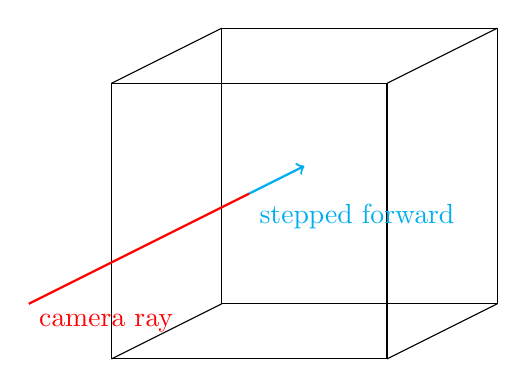
\begin{tikzpicture}[scale=0.7]
        \draw (0,0) -- (5,0) -- (5,5) -- (0, 5) -- (0, 0);
        \draw (2,1) -- (7,1) -- (7,6) -- (2, 6) -- (2, 1);
        \draw (0,0) -- (2,1); \draw (5,0) -- (7,1); \draw (5,5) -- (7,6); \draw (0,5) -- (2,6); 
        \draw[thick,red] (-1.5,1) node[below right]{camera ray} -- (2.5,3);
        \draw[->,thick,cyan] (2.5,3) node[below right]{stepped forward} -- (3.5,3.5);
    \end{tikzpicture}
    \caption{A ray is created from the camera to the object. From there, it is extended into the volume.}
\end{figure}

\pagebreak
\noindent
In ray marching, the algorithm only knows when it has reached the surface, or to be precise when it is inside the actual object volume.
\\
With this information, it is only possible to extend the ray in steps of a predefined length until the inside of the object is reached.
Traditional ray marching then tries to approximate the surface distance by stepping back (and by that out of the surface) and forward repeatedly in continuously smaller steps, thus converging towards the exact distance.
\\
Once the step size falls below a certain threshold, the distance approximation is assumed to be precise enough and the value is returned for that ray march.

\begin{figure}[H]
    \centering
    \begin{tikzpicture}[scale=1.2]
        \tikzset{edge/.style = {-{Latex[length=3mm]}}}
        \tikzset{smalledge/.style = {-{Latex[length=2mm]}}}

        % ray
        \draw[edge] (0,2) node[above,sloped,xshift=1cm]{ray} -- (10,3);
        \node (1) at (2,2.2) {\textbullet};
        \node (2) at (4,2.4) {\textbullet};
        \node (3) at (6,2.6) {\textbullet};
        \node (4) at (8,2.8) {\textbullet};

        % surf dist
        \draw[red] (2,1.5) -- (2.5,2) -- (4,1.8) -- (5,1.5) -- (7.4,2) -- (7.7,4) -- (9,4.3);

        % reverse nodes
        \node[cyan] (5) at (7,2.7) {\textbullet};
        \node[cyan] (6) at (7.5,2.75) {\textbullet};

        % ray steps
        \draw[edge] (1) edge[bend left=90] node [left]{} (2);
        \draw[edge] (2) edge[bend left=90] node [left]{} (3);
        \draw[edge] (3) edge[bend left=90] node [left]{} (4);

        % rey reverse steps
        \draw[smalledge,cyan,shorten >=-0.1cm,shorten <=-0.1cm] (4) edge[bend left=90] node [left]{} (5);
        \draw[smalledge,cyan,shorten >=-0.1cm,shorten <=-0.1cm] (5) edge[bend left=90] node [left]{} (6);

        % close enough
        \draw[cyan, shorten <=-0.2cm] (6) -- (9,3.7) -- (11,3.7) node[xshift=-1cm,above]{close enough};
        
        \end{tikzpicture}
    \caption{The ray is stepped forward until the surface is reached and tries to step in and out of the object until the step size falls below a certain threshold.}
\end{figure}

\subsubsection{Sphere Tracing}
TODO.